\documentclass[lang=en,mode=normal,device=normal,color=blue,12pt]{elegantnote}

\usepackage{amsmath,amssymb}
\usepackage{bbm}
\usepackage{tcolorbox}
\usepackage{graphicx}
\usepackage{booktabs}
\usepackage{subfig}
\usepackage{algorithm}
\usepackage{algpseudocode}
\usepackage[toc,page,title]{appendix}
\usepackage{hyperref}

\setlength{\parindent}{0pt}

\DeclareMathOperator*{\E}{\mathbb{E}}
\DeclareMathOperator*{\1}{\mathbbm{1}}
\DeclareMathOperator*{\R}{\mathbbm{R}}
\DeclareMathOperator*{\argmax}{arg\,max}
\DeclareMathOperator*{\argmin}{arg\,min}

\title{Study Note: Proximal Policy Optimization}

\author{Yanqing Wu\\[0.5cm]{Advisor: Prof. Hengshuai Yao}}
\institute{Viwistar Robotics}

\begin{document}
\maketitle

\newpage

% PPO: first-order method, on-policy learning, actor-critic structure

Since some parts are not addressed directly from the literature, the explanations in this note are the best of my understanding.

\section{Introduction}

In normal policy gradient, training can be unstable due to sparse reward and sampled target, causing dramatic changes on the policy; this eventually collapses performance.
To enhance training stability, we want to limit the parameter updates that would change the policy too much at one step\footnote{In supervised learning, it will be corrected on the next update. In RL, step too far results in terrible policy and new data will be collected in this policy, therefore cannot be self-corrected.}.
With this goal, True Region Policy Optimization (TRPO) \cite{schulman2017trust} was introduced.
TRPO delimit the KL-divergence with a constraint. More specifically, TRPO updates policies by taking the largest step possible to improve performance while satisfying the constraint on how close the new and old policies are allowed to be \footnote{Trust Region is a more advanced \textit{step-sizing} method than line search along gradient}.
However, TRPO is complicated to implement and is computational-heavy (from the computation of second-order derivatives of KL-divergence). Proximal Policy Optimization (PPO) \cite{schulman2017proximal} simplifies it by using a \textit{clipped surrogate objective} while retaining similar constraints and similar performance.
Instead of enforcing a hard constraint as in TRPO, PPO formalized the constraint as a penalty in the objective function.

There are two primary variants of PPO: PPO-Clip and PPO-Penalty.
\newline
\textbf{PPO-Clip} does not have a KL-divergence term in the objective and does not have a constraint at all. Instead relies on specialized clipping in the objective function to remove incentives for the new policy to drift from the old policy, PPO does hard clipping the policy ratio to be within a small range around 1.0, where 1.0 means the new policy is the same as old.
\newline
\textbf{PPO-Penalty} approximately solves a KL-constrained update like TRPO, but penalizes the KL-divergence in the objective function instead of making it a hard constraint, and automatically adjusts the penalty coefficient throughout training so that it is scaled appropriately.
PPO-Penalty performs worse than PPO-Clip \cite{schulman2017proximal}.

% PPO combines ideas from A2C (having multiple workers) and TRPO (it uses a trust region to improve the actor).
%The main idea is that after an update, the new policy should be not too far from the old policy. For that, PPO uses clipping to avoid too large updates.






\section{Implementation}


% https://towardsdatascience.com/proximal-policy-optimization-tutorial-part-1-actor-critic-method-d53f9afffbf6
% https://towardsdatascience.com/proximal-policy-optimization-tutorial-part-2-2-gae-and-ppo-loss-fe1b3c5549e8
PPO uses the Actor-Critic approach. It uses two models, Actor Model and Critic Model, as shown in Figure \ref{fig:ppo_ac}.

% TODO: use tikz
\begin{figure}[!ht]
  \centering
  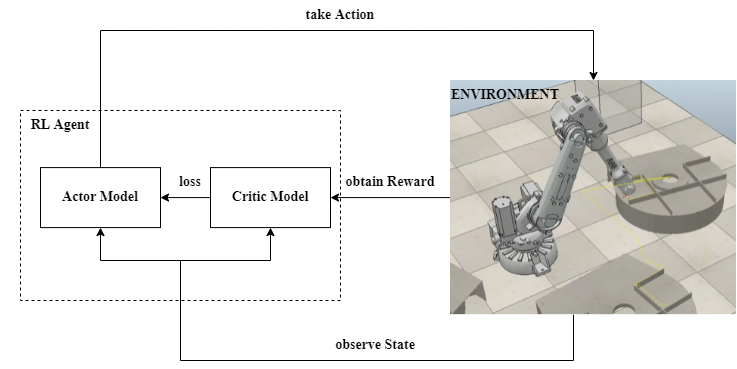
\includegraphics[width=0.9\linewidth]{PPO_AC.PNG}
  \caption{PPO agent}
  \label{fig:ppo_ac}
\end{figure}

The Actor model (policy $\pi$) learns what action to take under a particular observed state of the environment.
% In our case, it may take joint angles, obstacle positions and/or collisions as inputs and gives tip pose as action for output. 
The action predicted by the actor is sent to the environment. Afterwards, observation is made and reward is given from the environment and fed into the Critic Model.

The Critic model (value $V(s)$) learns to evaluate changes in the environment after action is taken by the Actor, and gives its feedback to the Actor. It outputs a real number indicating a rating (Q-value) of the action taken in the previous state. By comparing this rating obtained from the Critic, the Actor compares its current policy with a new policy and decides how it wants to improve itself to take better actions.



\subsection{OpenAI PPO}

\begin{figure}[!h]
  \centering
  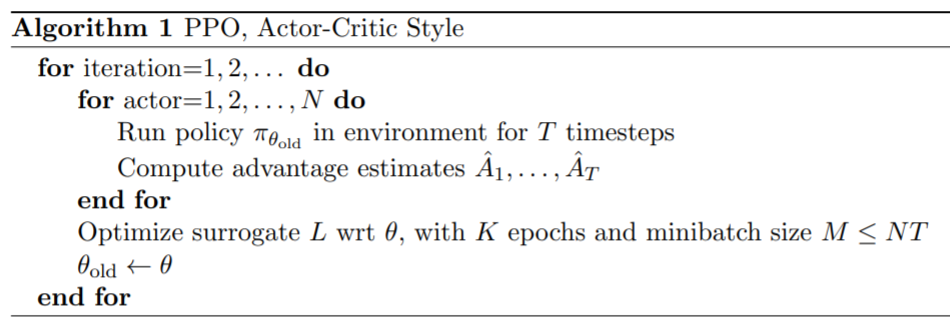
\includegraphics[width=0.7\linewidth]{ppo_openai.PNG}
  \caption{Screenshot of OpenAI PPO algorithm}
  \label{fig:ppo}
\end{figure}



\subsubsection{Key components}

Policy loss, value function loss, KL loss (optional) and entropy regularization make up the loss for PPO.

\textbf{Probability Ratio} $r_t(\theta)$ calculates how much the policy has changed. This ratio decides the tolerance of a change in policy. A clipping parameter epsilon $\epsilon$ is used to ensure only the maximum of $\epsilon$ change is made to the policy at a time. $r_t(\theta) > 1$ means the action is more probable for the current policy than the old policy.
\[
r_t(\theta) = \frac{\pi_{\theta} (a_t | s_t)}{\pi_{\theta_\text{old}} (a_t | s_t)} = \frac{\pi_{new}(\theta)}{\pi_{old}(\theta)} \overset{\mathrm{\text{computational convenience}}}= e^{ log(\pi_{new}(\theta)) - log(\pi_{old}(\theta)) }
\]


% https://stackoverflow.com/questions/46422845/what-is-the-way-to-understand-proximal-policy-optimization-algorithm-in-rl
% A-hat could be the discounted return (as in REINFORCE) or the advantage function (as in GAE) for example
\textbf{Advantage} $\hat{A}$ measures how much better or worse by taking a particular action in a particular state. Advantage is computed using Generalized Advantage Estimator (GAE($\lambda$)). Truncated version of advantage estimator $\hat{A_t}$ is given by
\begin{align*}
\hat{A_t} & = \delta_t + (\gamma \lambda)\delta_{t+1} + \cdots + (\gamma\lambda)^{T-t+1}\delta_{T-1} \\
\delta_t & = r_t + \gamma V(s_{t+1}) - V(s_t)
\end{align*}

\textbf{Actor Loss}, or \textbf{Policy (Gradient) loss} $L^{CLIP}$ is defined as a minimum of two functions in PPO. The first function $p_1$ is a surrogate loss function from conservative policy iteration ($L^{CPI}$), which is from TRPO \cite{schulman2017trust}.
The second function $p_2$ is the clipped probability ratio, which $r_t(\theta)$ is limited within the interval $[1-\epsilon, 1+\epsilon]$ ($\epsilon$ is clipping range).
The minimum of the two is taken so that the final objective is a lower bound (i.e. a \textit{pessimistic bound}) on the unclipped objective.
\begin{align*}
p_1 & = \text{ratio}\cdot\text{advantage} = r_t(\theta)\cdot\hat{A_t}\\
p_2 & = \text{clip}(\text{ratio}, 1-\epsilon, 1+\epsilon)\cdot\text{advantage} = clip(r_t(\theta), 1-\epsilon, 1+\epsilon)\cdot\hat{A_t}\\
L^{CLIP}(\theta) & = min(p_1, p_2) = \hat{\E_t}[min(r_t(\theta)\hat{A_t},clip(r_t(\theta),1-\epsilon,1+\epsilon)\hat{A_t})]
\end{align*}

Based on my understanding from \cite{ppocs294}, to illustrate why the minimum of the two functions is chosen, see Figure \ref{fig:mm_algo} below.
\begin{figure}[!ht]
  \centering
  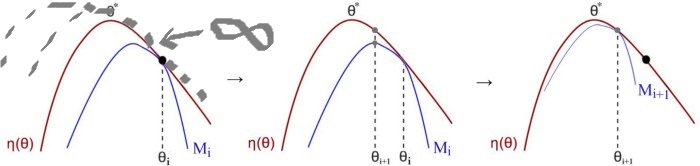
\includegraphics[width=0.9\linewidth]{MM_lowerbound.jpeg}
  \caption{Minorize-Maximization (MM) Algorithm}
  \label{fig:mm_algo}
\end{figure}
Think of the red line as a true objective function, and the blue line as a local approximation.
If we choose to maximize all the way, the approximation will go to infinity.
If we take local approximation and subtract a penalty, we receive a lower bound on the true objective function.
When we make progress on this pessimistic version of the objective, we are guaranteed to make progress and eventually converge on the true objective function . The idea behind this is Minorize-Maximization Algorithm.
Alternatively by \cite{weng2018PG}, the minimum is chosen because we avoid increasing the policy update to extremes for better rewards.

Policy loss correlates to how much the policy (process for deciding actions) is changing.
The magnitude of this should decrease during a successful training session.
These values will oscillate during training. Generally they should be less than 1.0.


Another version of $L^{CLIP}$ is as follows:
$$ L(s,a,\theta_k,\theta) = \min\left(
\frac{\pi_{\theta}(a|s)}{\pi_{\theta_k}(a|s)}  A^{\pi_{\theta_k}}(s,a), \;\;
g(\epsilon, A^{\pi_{\theta_k}}(s,a))
\right) $$
where $g(\epsilon,A) = (1+\epsilon)A$ when $A \geq 0$ and $g(\epsilon,A) = (1-\epsilon)A$ when $A < 0$. Through some simplifications, we see that probability ratio $\frac{\pi_{\theta}(a|s)}{\pi_{\theta_k}(a|s)}$ is clipped at $1+\epsilon\;(A>0)$ and $1-\epsilon\;(A<0)$. The hyperparameter $\epsilon$ specifies how much the new policy is allowed to change from the old policy (while still profiting the objective). Therefore, the clipping acts as a regularizer by discouraging the policy to change dramatically (see Figure \ref{fig:lclip}).

\begin{figure}[!ht]
  \centering
  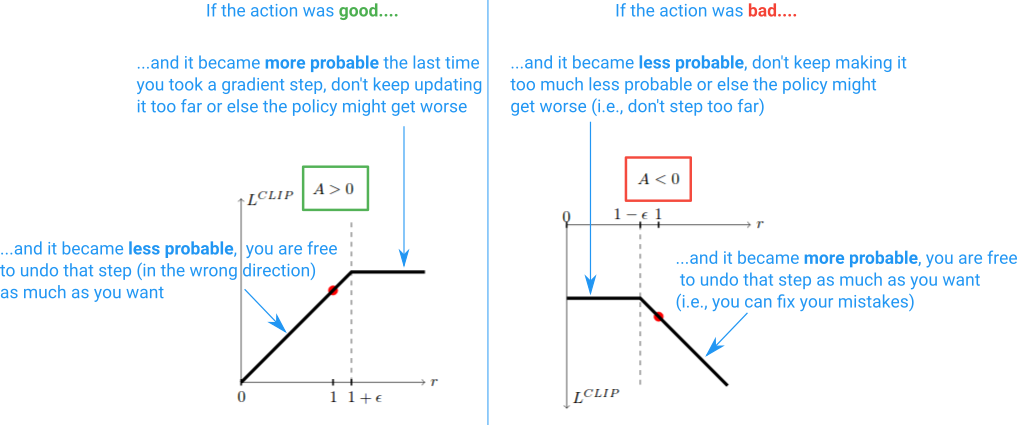
\includegraphics[width=0.9\linewidth]{LCLIP.PNG}
  \caption{Effect of $L^{CLIP}$ function \cite{ppolclip}}
  \label{fig:lclip}
\end{figure}

\textbf{Critic Loss}, or \textbf{Value (Function) Loss} $L^{VF}$ is defined as mean squared error between critic values and returns (or $V_t^{target}$ in the paper).
Target value is computed using TD($\lambda$) estimator.
Value Loss correlates to how well the model is able to predict the value of each state.
This should increase while the agent is learning, and then decrease once the reward stabilizes.
These values will increase as the reward increases, and then should decrease once reward becomes stable.
\[
L^{VF} = (V(s) - R)^2 = (V_\theta(s_t) - V_t^{target})^2
\]

\textbf{Total Loss}, or \textbf{Objective Loss} $L_t^{CLIP+VF+S}$ is defined as\footnote{The plus/minus sign of each loss component differs from source to source. The sign of the first (text) equation is align with PPO2 source code and some online post; the sign of the second (letter) equation is align with the paper.}\footnote{Based on discussion with the Advisor, the plus/minus sign of the first (text) equation should be the correct version. We must maximize entropy to minimize loss, hence the minus sign before entropy.}:
\begin{align*}
\text{total loss} & = \text{actor loss} + \text{critic loss} - \text{entropy} \\
L_t^{CLIP+VF+S}(\theta) & = \hat{\E_t} [L_t^{CLIP}(\theta) - c_1 L_t^{VF} + c_2 S[\pi_\theta](s_t)]
\end{align*}
where $c_1, c_2$ are coefficients, $\theta$ is a vector of policy parameters, $S$ is entropy bonus that acts as a regularizer to encourage policy exploration (see Appendix \ref{appendix:entropy} for more information of \textit{Entropy}).

Note that actor loss ($L_t^{CLIP}$) and critic loss ($L_t^{VF}$) correspond to exploitation, and entropy regularization ($S$) corresponds to exploration. The total loss equation here is a trade-off problem between exploitation and exploration, which is one of the key features and challenges in RL problems.


\subsubsection{Practical considerations}

There are two alternating threads in PPO. In the first thread, policy interacts with the environment, collects data and computes advantage estimates (using fitted baselines estimates); in the second thread, it collects all the experiences and runs Stochastic Gradient Descent (SGD) to optimize the policy using the clipped objective.

The surrogate loss $L$ is optimized with minibatch SGD on $NT$ timesteps of data, where $N$ is the number of parallel actors and $T$ is timesteps.



\subsection{DeepMind PPO}

DeepMind paper provides a more detailed pseudocode than OpenAI. According to DeepMind pseudo-code of PPO (\ref{fig:ppo})

\begin{figure}[!ht]
  \centering
  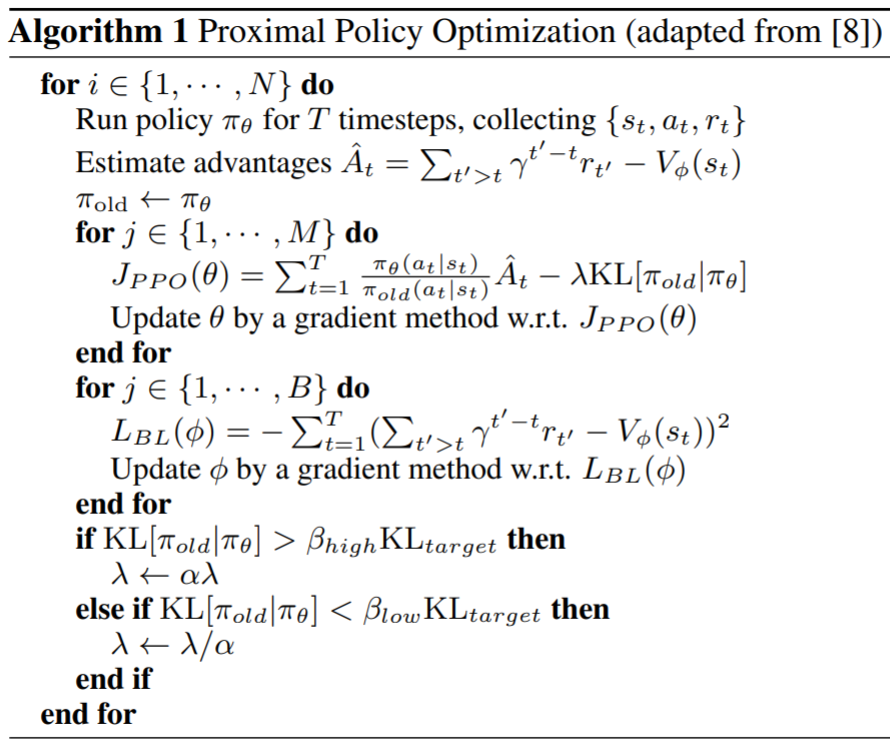
\includegraphics[width=0.7\linewidth]{ppo.PNG}
  \caption{Screenshot of DeepMind PPO algorithm}
  \label{fig:ppo}
\end{figure}

In this algorithm, $KL_{target}$ is the desired change in the policy per iteration.
The Actor maximizes $J_{PPO}$, and Critic minimizes $L_{BL}$.

\section{PPO Improvement}

In a later paper by \cite{hsu2020revisiting}, two common design choices in PPO are revisited, precisely (1) clipped probability ratio for policy regularization and (2) parameterize policy action space by continuous Gaussian or discrete softmax distribution. They first identified three failure modes in PPO and proposed replacements for these two designs.

The failure modes are:
\begin{itemize}
\item On continuous action spaces, standard PPO is unstable when rewards vanish outside bounded support.
\item On discrete action spaces with sparse high rewards, standard PPO often gets stuck at suboptimal actions.
\item The policy is sensitive to initialization when there are locally optimal actions close to initialization.
\end{itemize}


Discretizing the action space or use Beta distribution helps avoid failure mode 1\&3 associated with Gaussian policy. Using KL regularization (same motivation as in TRPO) as an alternative surrogate model helps resolve failure mode 1\&2.




%%%%%%%%%%%%%%%%%%%%%%%%%%%%%%%%%%%%%%%%%%%%%%%
% Appendices
%%%%%%%%%%%%%%%%%%%%%%%%%%%%%%%%%%%%%%%%%%%%%%%

\newpage
\begin{appendices}

\section{Entropy}
\label{appendix:entropy}

Entropy was first recognized in classical thermodynamics and was brought to information theory by Claude Shannon in the mid 20th century. It is now widely used and is most commonly associated with a state of disorder, randomness, or uncertainty.
In the realm of machine learning, entropy is related to randomness in the information being processed in a system. In other words, high entropy means that the randomness in the system is high, meaning it is difficult to predict the state in it. More specifically, in reinforcement learning (RL), entropy refers to the unpredictability of the actions taken of an agent. The more uncertain of which action will be taken by the agent, the higher the entropy. An example can be seen below in Figure \ref{fig:entropy}.

\begin{figure}[!htbp]
  \centering
  \subfloat[Discrete probability distribution $p(a|s)$]{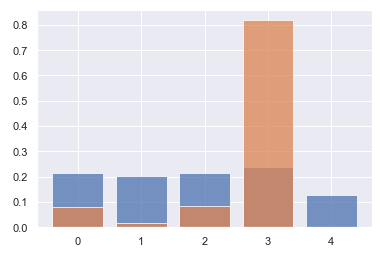
\includegraphics[width=0.5\textwidth]{entropy_discrete.PNG}\label{fig:entropy_discrete}}
  \hfill
  \subfloat[Continuous probability distribution $p(a|s)$]{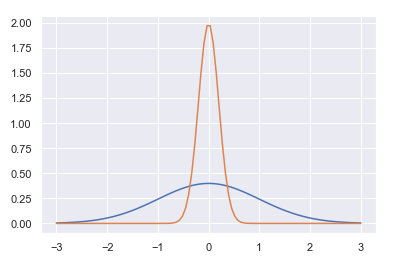
\includegraphics[width=0.5\textwidth]{entropy_cts.PNG}\label{fig:entropy_cts}}
  \caption{Orange shows low-entropy distributions. Blue shows high-entropy distributions.}
  \label{fig:entropy}
\end{figure}



\subsection{Terminology}

Based on my understanding of RL literature, `entropy' technique in RL normally refers to `entropy regularization'. `entropy regularization' technique includes but not limited to adding `entropy bonus' in objective function and using `maximum-entropy'. `entropy bonus' includes but not limited to `one-step (naive) entropy bonus' and `proper entropy bonus'. The term `entropy bonus' is usually a constant or a vector of real numbers. `one-step entropy bonus' only applies to the current state, while `maximum-entropy' optimizes over the long-term sum of entropy. There is also a technique to maximize over both long-term rewards and long-term entropy. This is referred to as maximum entropy reinforcement learning.



\subsection{Why use entropy in RL}

It is a common practice to use entropy regularization to ensure policy exploration in policy gradient methods \cite{odonoghue2017combining}.
An agent might be stuck in a local optimum or never finding the global optimum because of not exploring the behavior of other actions.
Entropy encourages exploration, avoiding the situations where agent might fall into a local optimum.
This is critical for tasks with sparse reward because the agent seldomly receives feedback for its action, and therefore might overestimate some reward received and repeat the actions that led to that reward. With improved exploration, the agent will be more robust to abnormal or rare events while developing a task.

Other benefits of using entropy includes augmenting RL objective \cite{brianEntropy2010}, encouraging longer episodes \cite{schulman2018equivalence}, fine-tuning policies and better adaptability to new environments \cite{haarnoja2017reinforcement}.



\subsection{How to use entropy in RL}

In information theory, entropy for a discrete random variable $x$ is defined as: 
\begin{equation}
\label{eqn:info_entropy}
H(X) = -\sum_{x\in X} P(x) logP(x)
\end{equation}
In RL, the formula becomes Equation \ref{eqn:rl_discrete_entropy} as we calculate the entropy of the policy $\pi(a|s_t)$ for discrete action space (replace sum with integral for continuous action space).
\begin{equation}
\label{eqn:rl_discrete_entropy}
H(\pi(\cdot|s_t)) = -\sum_{a\in \mathcal{A}} P(x) log P(x)
\end{equation}

It is typical to add an `entropy bonus' term to the loss function, which encourages the agent to take actions more unpredictably so as to counteract the tendency of falling into local optimum \cite{odonoghue2017combining}.
For example, in A3C \cite{mnih2016asynchronous}
\[
\nabla_{\theta'}log\pi (a_t | s_t; \theta')(R_t - V(s_t;\theta_v))+\beta\nabla_{\theta'}H(\pi(s_t;\theta'))
\]
where $H(\pi)$ is the entropy bonus term, and the hyperparameter $\beta$ controls the strength of the entropy regularization term. \cite{mnih2016asynchronous} found that adding the entropy of the policy $\pi$ to the objective function improved exploration by discouraging premature convergence to suboptimal deterministic policies.

For one more example, \cite{schulman2018equivalence} discussed naive and proper entropy bonuses for A2C (advantage actor critic; a well-tuned version of A3C). The entropy bonus term is added in following way:

naive / one-step entropy bonus:
\[
\nabla log \pi_\theta (a_t | s_t) \bigg( \sum_{d=0}^{n-1} \gamma^d r_{t+d} - V(s_t) \bigg) - \tau \nabla_\theta \underbrace{ D_{KL} [\pi_\theta || \bar{\pi} ] (s_t)}_\text{entropy bonus}
\]

proper entropy bonus:
\[
\nabla log \pi_\theta (a_t | s_t) \bigg( \sum_{d=0}^{n-1} \gamma^d (r_{t+d} - \tau \underbrace{ D_{KL}[\pi_\theta || \bar{\pi}](s_{t+d})}_\text{entropy bonus} ) - V(s_t) \bigg) - \tau \nabla_\theta \underbrace{ D_{KL} [\pi_\theta || \bar{\pi} ] (s_t) }_\text{entropy bonus}
\]

A side note for training: entropy should slowly and consistently decrease during a successful training process. If it decreases too quickly, the entropy coefficient hyperparameter should be increased.


\subsection{Further reading}

Application of entropy (regularization) in RL is a well-studied topic, some notable paper in this area:

\begin{itemize}
\item \cite{ahmed2019understanding} Understanding the impact of entropy on policy optimization
\item \cite{schulman2018equivalence} Equivalence Between Policy Gradients and Soft Q-Learning
\item \cite{haarnoja2017reinforcement} Reinforcement Learning with Deep Energy-Based Policies (soft (entropy-regularized) Q-learning)
\item \cite{nachum2017bridging} Bridging the Gap Between Value and Policy Based Reinforcement Learning (entropy bonus)
\item \cite{odonoghue2017combining} Combining policy gradient and q-learning (entropy bonus)
\item \cite{mnih2016asynchronous} Asynchronous Methods for Deep Reinforcement Learning (A3C)
\item \cite{brianEntropy2010} Modeling purposeful adaptive behavior with the principle of maximum causal entropy
\item \cite{Williams1992SimpleSG} Simple statistical gradient-following algorithms for connectionist reinforcement learning
\end{itemize}

Related topics include one-step entropy vs. maximum entropy, and entropy vs. KL-divergence as regularizer.

\newpage
\section{PPO1 vs. PPO2}

PPO2 is made for GPU by OpenAI. It uses vectorized environments for multi-processing while PPO1 uses MPI. PPO2 contains several modifications from the original algorithm which are not documented by OpenAI: value function is also clipped and advantages are normalized \cite{ppo2stable}.

PPO1 is not gpu-optimized: it uses one environment per MPI worker. In other words, when running PPO1 with multiple MPI processes, each process creates its own copy of the environment, and its own neural net (NN). The gradients for NN updates are aggregated across the workers by virtue of using MpiAdamOptimizer class.
PPO2 implementation (while with recent updates it can use MPI as well) uses a different version of parallelism. Head process with a single neural net creates a bunch of subprocesses that run separate environments (run environments means that take actions and produce next observations and rewards).
The observations and rewards from these multiple environments in subprocesses are batched together in the head process.
For visual observations, that creates a big enough batch so that computation of NN gradients on a GPU starts making sense.
By default, multiple environments in subprocesses are only used for atari and retro video games, but not, for instance, for mujoco (because observations there are not visual) \cite{ppo2vsppo1}.

In conclusion, PPO1 is obsolete at the time of writing this note, and its functionality is fully covered by PPO2.

\subsection{OpenAI source code of PPO}

\begin{itemize}
\item PPO1: \url{https://github.com/openai/baselines/blob/master/baselines/ppo1/pposgd_simple.py}
\item PPO2: \url{https://github.com/openai/baselines/blob/master/baselines/ppo2/model.py}
\end{itemize}

\end{appendices}


%%%%%%%%%%%%%%%%%%%%%%%%%%%%%%%%%%%%%%%%%%%%%%%
% References
%%%%%%%%%%%%%%%%%%%%%%%%%%%%%%%%%%%%%%%%%%%%%%%

\newpage
\bibliography{references_PPO}


\end{document}
















